\section{Iteración III}
\subsection{Resumen}
En ésta iteración se realizó el frontend del login de ARF así como el backend para los módulos ``LOGIN", ``REGISTRAR CUENTA" y ``GUARDAR ESCENARIO" de acuerdo a la arquitectura descrita en la figura 4.25. \par

%\subsection{Diagramación}
\subsection{Desarrollo}
El desarrollo de los módulos de backend mencionados se realizó sobre Lambdas de AWS. Cada módulo tiene su propia función. El objetivo de hacerlo de esta forma es brindarle escalabilidad al sistema pues el desarrollo se logra de forma modular.\par
Cada uno de estos módulos es accesible a través del protocolo HTTP gracias a la API Gateway. La API Gateway es un módulo de Amazon Web Services que permite que los recursos de AWS sean accesibles desde el exterior, en éste caso, permite que la aplicación en Android pueda acceder a estas funciones con una simple petición. Asimismo las imágenes de los escenarios son almacenadas en AWS S3.\par

\subsubsection{Login}
Se encarga de la funcionalidad del login de la aplicación. En la figura 4.29 se puede observar el diagrama del proceso de login.\par
\begin{figure}[h!]
	\centering
	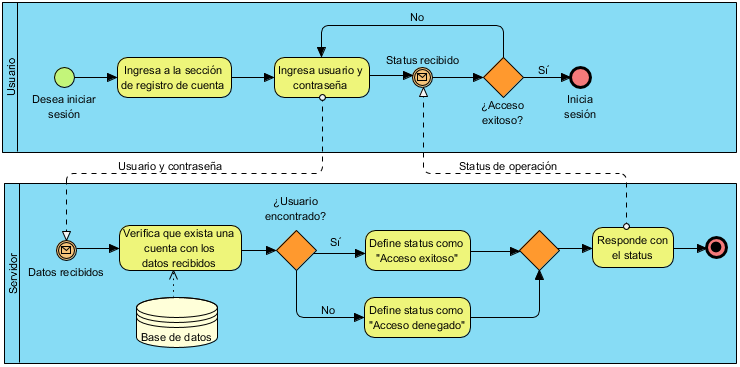
\includegraphics[width=15cm,height=9cm]{imagenes/desarrollo/diagramas/BPMN_LOGIN.png}
	\caption{Diagrama de proceso de Login.}
	\label{fig:loginsuccess}
\end{figure}

\subsubsection{Registro}
Ésta función se encarga de registrar un nuevo usuario en la base de datos para que posteriormente pueda iniciar sesión en la aplicación. El modelado de este proceso se puede apreciar en la figura 4.30. \par
\begin{figure}[h!]
	\centering
	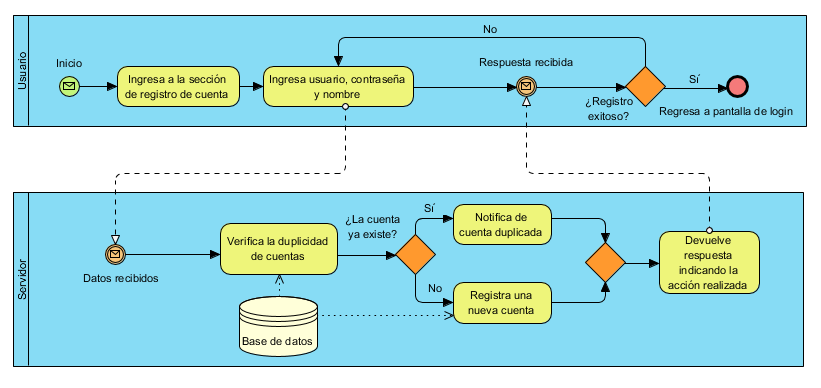
\includegraphics[width=15cm,height=7cm]{imagenes/desarrollo/diagramas/BPMN_REGISTRAR_CUENTA.png}
	\caption{Proceso de registro de nuevo usuario.}
	\label{fig:regsuccess}
\end{figure}
\par

\subsubsection{Guardar escenario}
El objetivo de ésta función es poder almacenar los escenarios que vayan generando los usuarios para que después puedan ser visualizados desde la aplicación. En la figura 4.31 se puede apreciar el modelado del proceso de almacenamiento de escenario. \par
\begin{figure}[h!]
	\centering
	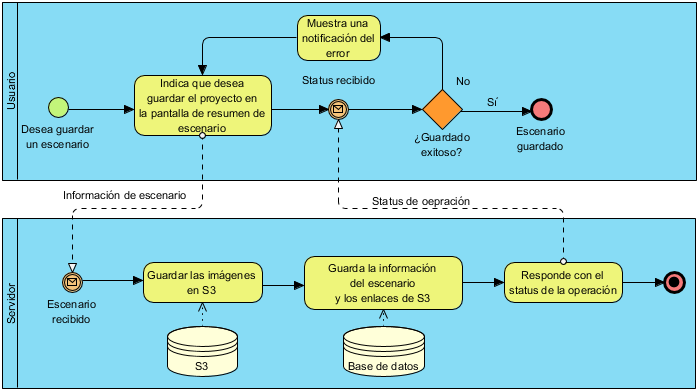
\includegraphics[width=13cm,height=7cm]{imagenes/desarrollo/diagramas/BPMN_STORESC.png}
	\caption{Proceso de guardado de escenario.}
	\label{fig:regsuccess}
\end{figure}
\clearpage